Cryptography plays a vital role in securing communication. The use of cryptographic techniques for securing communication between two parties could be traced back up to the ancient time of starting conversation itself. In those ancient times, very fundamental techniques like carrier pigeons or predefined codes and signals were used for achieving security in the communication. It is evident that those schemes have a lot of drawbacks but the idea itself of securing communication between two parties in such a way that no one other than themselves, can understand their conversation, was the foundation of cryptography. In the early days of cryptography, very fundamental techniques such as substitution or permutation algorithms were used, where the key was used for deciding the values of substitution or permutation. In those days, not only the key but also the algorithm of cryptography was kept a secret so no intruder can decipher their messages by performing cryptanalysis on encrypted message. 

This system persisted up to the 19th century until Kerckhoffs principle was widely accepted. The principle stated that a cryptosystem should remain secure when only the key is secure, and all other elements of that system like its algorithm are public knowledge. This principle actually set up a mathematical basis for modern cryptosystems. Those crypto systems need to be proved reliable on the mathematical basis and principles to be called secure. The symmetric cryptosystems which use a single key for encryption, as well as decryption, was providing confidentiality and the MAC\nomenclature{MAC}{Message authentication code} provides the Data integrity of the text, but those systems did not implement other security services.

In 1976, Diffie-Hellman proposed the concept of public key cryptography. Their idea was the use of different keys for encryption and decryption. In their design, the public key of the receiver was used for encryption and the private key of receiver used for decryption of the message. This idea could answer a fundamental problem of secure key exchange. Later the RSA and ElGamal cryptosystem bring the public key cryptography in reality and widely used up until the present. The public key cryptosystem was subsequently devised into the formation of digital signatures which are substituting the physical handwritten signatures and allowing to sign electronically. The digital signatures used along with HMAC\nomenclature{HMAC}{keyed-hash message authentication code} achieve most of the security services. The following section describes the security services and their need.

\section{Security Services}
Security services\index{security services} are the services which ensure that adequate security is provided by a cryptosystem to maintain its security. Every cryptosystem has its own strengths and weaknesses. The security services are a good measurement for measuring the strengths and weaknesses of a cryptosystem. A cryptosystem needs to mathematically prove that it provides multiple security services for establishing its security capability. A cryptosystem providing a particular set of security services is capable of defending attacks for which the security service was defined. The following section describes some important security services which a group signature scheme must provide.
 
\subsection{Confidentiality} 
The confidentiality\index{confidentiality} is a security service which provides protection against passive attacks. The purpose of the confidentiality is to allow access to only those who have the privilege to access the information. Those who do not have such privilege should not have access to the information. Privacy is one of the important concepts in confidentiality. Privacy must be maintained in the system appropriately so an unauthorized person must not access any private information. The privacy is utmost important in real world scenario. If a system does not maintain privacy, then the user of the system will not feel secure while using the system. Confidentiality is primarily maintained by encrypting private information using a cryptographic algorithm and providing the decryption key to only those who have the privilege to access the information.
\subsection{Integrity}
Data integrity\index{integrity} is a security service, which is used for detection of an active attack. In active attacks, the contents of the communication are altered by an attacker. The data integrity provides assurance to the receiver that the data was not modified during transmission and arrived exactly same as sent by the sender. During transmission, it is possible that the data can be changed accidentally or intentionally. The accidental data modification can be occurred due to noise in transmission, but those changes are minimal and can be recovered using error correction techniques. An active attack also leads to modification of data. This modification is precise and deliberate so it must be detected. An ideal integrity checking algorithm should be able to detect substitution, permutation, insertion or deletion of bits or characters of the message. Integrity checking is done by creating a fixed size message digest and transmitting it along with the message and receiver validates the digest by comparing it with recreated digest from received message. The hashing algorithm provides a good solution for integrity checking and some of the hashing algorithm working almost ideally like SHA256.
\subsection{Authenticity}
The purpose of authentication\index{authentication} is validating the source of a message as it is what it claims to be. A secure cryptosystem must have authentication as a security service. In the absence of authentication procedure in a system, it is easily possible for an attacker to masquerade as an authorized user. There are mainly three types of information which can be used for authentication.

First is information only legitimate user knows. This kind of data can be PIN\nomenclature{PIN}{Personal Identification Number}, password or a private key. This information should only be known to the user and if this information gets leaked then entity possessing its knowledge can masquerade. Great care required to be taken during designing the system so this information must not be leaked. The second type is something user have. This type contains ID\nomenclature{ID}{Identification} proofs or encrypted swipe cards. The card contains user information and its key only known to the legitimate user. It provides additional protection as the card or key individually have no use for authentication, but a pair of both required for authentication. The third type of information is something a user is. It contains unique biometric traits that cannot be duplicated. Those traits can be fingerprint, retina scan or voice. Such features are almost impossible to replicate and hence considered most secure for authentication.  
\subsection{Non-repudiation}
The Non-repudiation\index{non-repudiation} service provides the proof of communication in a system. The meaning of the term non-repudiation means undeniability. The non-repudiation service prohibits an entity to deny its previous actions. The main two types of non-repudiation are Source non-repudiation and Destination non-repudiation. In source non-repudiation, a receiver can prove that specific sender sent a particular message so the sender cannot deny his action. In destination non-repudiation, the sender can confirm that the receiver, in fact, received a particular message. Usually, a trusted third party is required for implementing non-repudiation, but some cryptographic algorithm like Group Signatures and Digital Signatures could provide source non-repudiation service. 
\section{Authentication using Digital Signatures}
Digital signatures are well known for their application in cryptographic authentication. The digital signatures are viewed as a replacement of handwritten signatures for electronic documents. The digital signatures are implemented by using asymmetric public key cryptosystem. Next section provides a brief introduction to digital signatures with their use in public key infrastructure and discussion about privacy concerns in use of digital signatures.
\subsection{Digital Signatures}
The Digital signature\index{digital signatures} provides some exceptional security capabilities which are very difficult to accomplish in some other method. Digital signature substitutes handwritten signature in electronic documents and provides an ability to sign those documents. The system of Digital signature contains a signer and potentially many verifiers. The signer signs a document using his private key. 

The private key has a special mathematical relationship with the public key, and the private key is required to be kept secret or private to signer himself. It is evident from its name, the public key is made available, and it is accessible to any member of the system. The public key must require being unique so that it can uniquely determine the signer. The public key is used for verification of the signature. Asymmetric cryptography is used in the implementation of Digital signature, so it's hard to calculate private key from the public key, and the public key can only be used for decryption and not for encryption. The process of Digital signature consists of following three algorithms.
\subsubsection{Key Generation} 
The Key Generation algorithm executed initially by the user or a trusted key providing authority, which generates a pair of keys, i.e., a private key and a public key. These keys have some special mathematical relationship between them and cannot be substituted independently. The signer then keeps the private key protected and uses it to sign his documents and messages. The private key is made available to public and/or distributed to all potential verifiers.
\subsubsection{Signature Generation} 
When a user needs to sign a document or message, he can execute the signature generation algorithm, which takes the input of the private key, message and produces the signature for that message. The signer then attaches the generated signature along with the message as his sign and transmit it to the receiver.
\subsubsection{Signature Verification} 
By using signature verification algorithm, any verifier can check the validity of a signature. The signature verification takes the message, signature and signer's private key as input and produces a binary result that determines the validity of the signature.
 
Similar to a handwritten signature, the Digital signatures are extremely difficult to duplicate and protect signer from masquerade attack. A Digital signature algorithm required to implement following properties to prevent various attacks.
\begin{itemize}
\item A signature must be dependent on the message so it cannot be reused to forge a signature for other messages.
\item The algorithm must use signers unique information, or the public key must be unique to prevent forgery and also provides non-repudiation.
\item Both the signing and verification must require small computational overhead so that it should be easy to generate and verify a signature.
\item The Digital signature algorithm must provide proof that it is impossible to forge a signature.
\end{itemize} 

 \begin{figure}[h]
    \centering
    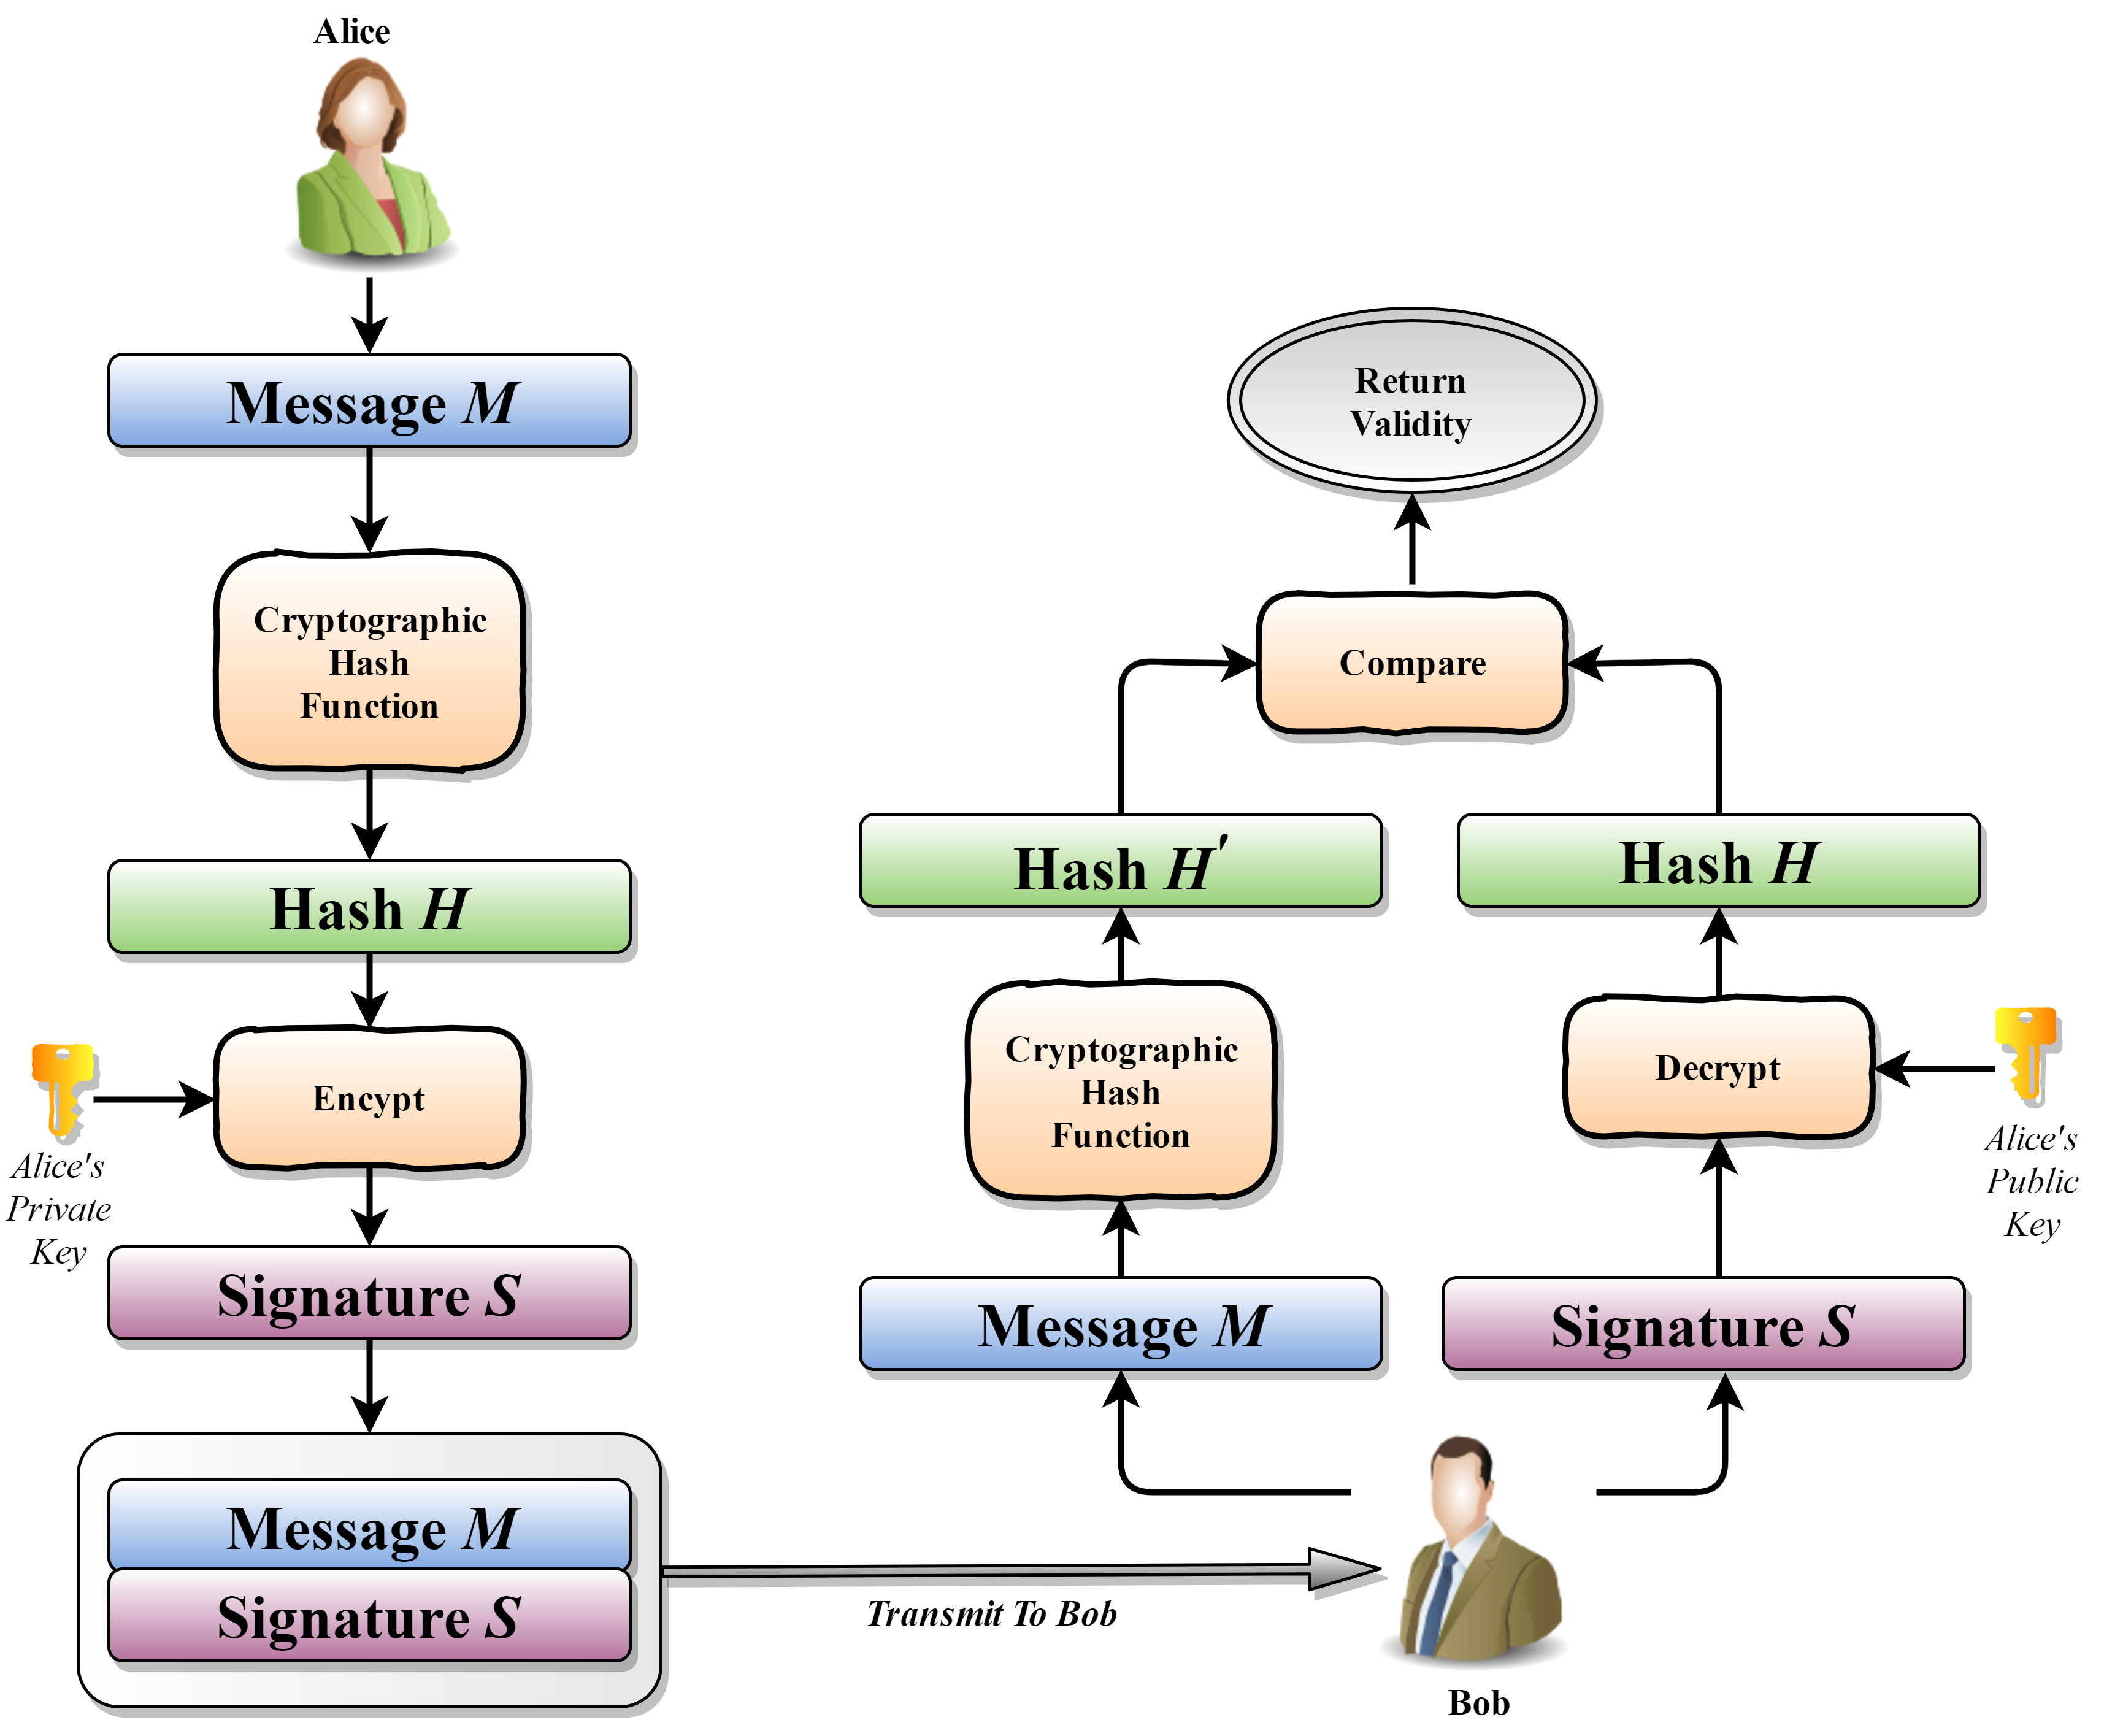
\includegraphics[width=\textwidth]{DigitalSignaturemod}
    \caption{Process of Digital Signature }
    \label{fig:Digital Signature}
\end{figure}

The figure \ref{fig:Digital Signature} shows the process of Digital signature. When Alice requires sending a message $M$, she first calculates hash $H$ of that message by using some predefined cryptographic hash function. The hash function produces a fixed size digest for a message which should be unique to avoid a collision. Then Alice encrypts the hash by using her private key and generates a signature $S$ for message $M$. The message $M$ along with signature $S$ is transmitted to the Bob, who is a potential verifier.

To verify the signature, Bob first calculates hash $H^\prime$ of the received message. Parallely he decrypts the signature $S$ by using Alice's public key, which should produce the hash $H$, which was calculated by Alice. Then Bob matches both the $H$ and $H^\prime$ and determines the validity of the signature which is true if $H = H^\prime$ and false if $H \neq H^\prime$. 

From the above example, we can analyze the security services provided by the Digital signatures. The collision resistant hash function produces unique digest for each message so the verifier can detect even a small change in the message. Hence the integrity is preserved in Digital signature. It is not possible to produce forged signature without knowing Alice's private key. Therefore verifier can rely on the authenticity of the message. The (private key, public key) pair is unique for Alice so she cannot deny her signature. Therefore the non-repudiation is also provided by Digital Signature. 

But along with the validity, Bob also gets to know the identity of Alice as her unique public key was used in validating the signature. As anyone can verify the signed message, the verifier also gets the identity of the signer and by using various messages signed by a signer can be used for profiling attack. Hence it is clear that the Digital signature does not provide confidentiality or privacy to the signer.
 
The Digital Signatures are widely used to ensure authenticity and already replacing traditional handwritten signatures. The RSA, ElGamal and Elliptic Curve algorithms are most popular asymmetric cryptographic algorithms used for Digital signatures. The Digital signatures are used in the field of web services and digital transactions along with signing electronic messages and documents.

\subsection{Public Key Infrastructure (PKI)}
Achieving authentication in a public key cryptosystem was one of the challenging problems. As a malicious user can easily masquerade as some other entity by using its public key. To overcome this problem, the concept of Public Key Infrastructure (PKI)\index{Public Key Infrastructure} \nomenclature{PKI}{Public Key Infrastructure} was introduced, which uses an application of Digital signatures. The PKI is a collection of policies and procedures required to create and manage digital certificates based on public key cryptography. The objective of PKI is to establish a relationship between an entity's cryptographic identity (e.g. public key) and non-cryptographic identities or attributes (like name, email, designation, etc.). Digital signatures are used in establishing such relationship. This link can be established using digital certificates by having trust between certified entity and issuer of the certificate. Using this certificate, a user can verify that the public key he is using for encryption, actually belongs to the entity which it claims to be. Masquerading as some other entity is not possible because the certificate can be easily validated in PKI. In short, the PKI solves the authentication problem in the public key cryptosystem. A simple Public Key Infrastructure includes following elements.
\subsubsection{Digital Certificate} A Digital Certificate\index{digital certificate} $cert_{CA \rightarrow A}$ is formed by PKI when it signs a message containing the cryptographic identity of $A$ (public key of $A$) and non-cryptographic identity of $A$ like its name. Whenever $A$ presents (public key of $A$, $cert_{CA \rightarrow A}$) to a verifier, the certificate can be verified that $cert_{CA \rightarrow A}$ is a valid signature generated by $CA$ using the public key of $CA$. The basic idea behind this is, $CA$ is a trusted by verifier that it will not certify invalid link between cryptographic and non-cryptographic identities. So $cert_{CA \rightarrow A}$ can be used to prove that the public key provided in the certificate $cert_{CA \rightarrow A}$, actually belongs to $A$. The Digital Certificate comes with an expiration time, and the certificate expires after that if it is not renewed.

\begin{figure}[h]
    \centering
    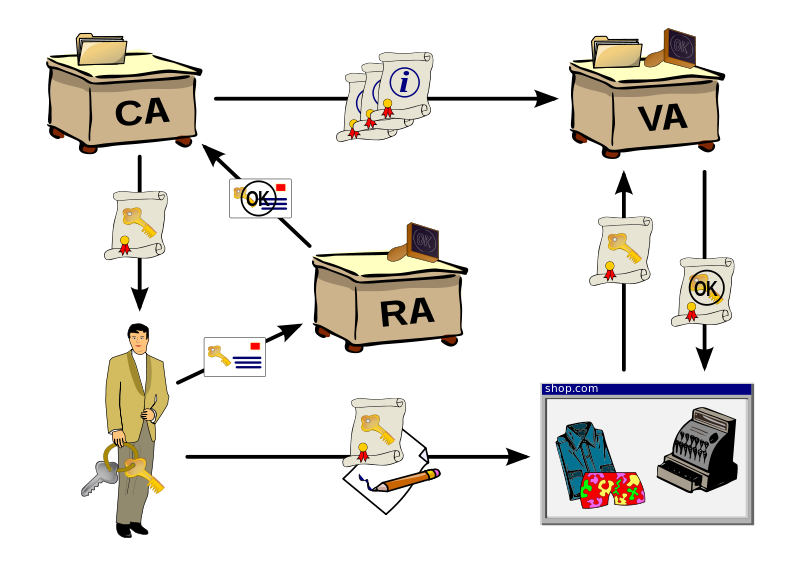
\includegraphics[width=\textwidth]{PKI}
    \caption{Public Key Infrastructure (PKI) }
    \label{fig:PKI}
\end{figure}

\subsubsection{Registration Authority (RA)} The fundamental objective of Registration Authority\index{registration authority(RA)} is to ensure valid registration of an entity. If an entity wants a digital certificate, then it required registering at registration authority. The registration authority verifies the validation of information provided to it and authenticate the entity making the request for the digital certificate. If everything is correct, then it sends a request to the Certificate Authority to issue a certificate for registered entity.
\subsubsection{Certificate Authority (CA)} The Certificate Authority\index{certificate authority(CA)} provides digital certificates to the entities enrolled by the Registration Authority. The Certificate Authority enables the user of PKI to rely on the public key in the certificate. It also acts as a trusted third party between the owner of a certificate and user on the certificate.
\subsubsection{Validation Authority (VA)} When a user of a certificate required to validate it, the Validation Authority\index{validation authority(VA)} provides validation. The Validation Authority receives all the certificate information from the Certificate Authority and used it to verify the certificate requested by the PKI user.\\
 
The PKI system also uses a certificate database which stores information of issued certificates, request for certificates and revoked certificates.

\subsubsection{Revocation of certificates} One of the important property of PKI is the ability to revoke any digital certificate which was issued in the past. There can be various reasons that a certificate required to be revoked. First is the expiration of time because each certificate has an expiration date and time. All the certificates which cross the expiration time and not renewed must be revoked after their expiration. Another reason is when the owner of a certificate changes his key, due to loss or theft of his private key. The certificate authority is responsible for the revocation of the certificate and sends the revocation information to validating authority so it can invalidate those certificates during verification.

\subsection{Privacy Issues}
In the earlier sections, we saw that the digital signatures provide security services like integrity, non-reputation, etc. The PKI also provides authentication by using trust-based systems. But while providing authenticity of the signer, digital signature or more generally PKI systems jeopardize user privacy. A digital signature of a user $A$ on some document $M$, when $A$ is in possession of PKI Certificate ($A$, public key of $A$, $cert_{CA \rightarrow A}$), reveals his identity to all the verifiers. Also when multiple of these digital signatures along with the signed messages by same user $A$, in different contexts, can be linked to him. It reveals much more information of the user. For example, a collection of multiple messages signed by the same user can be used for profiling of the signer. 
 
The PKI based authentication service provides one general solution to overcome this problem which is Anonymous Certificates. During generation of these anonymous certificates, CA verifies the identity of $A$, but the signature certificate $cert_{CA \rightarrow A}$ issued by CA on the public key of $A$, only contains (public key of $A$, $cert_{CA \rightarrow A}$). Where traditional certificates contain (non-cryptographic information of $A$, public key of $A$, $cert_{CA \rightarrow A}$). By using those anonymous certificates, it is not possible to obtain non-cryptographic information of a user directly from the certificate $cert_{CA \rightarrow A}$. But those anonymous certificates still provide the public key of a signer to all the verifiers. This information can be used to link a signer with the messages he signed and can be misused. 
 
The digital signatures and PKI certificates do not provide liberty to the user to maintain his privacy. The privacy of the user is sacrificed to obtain authenticity in those schemes. The next section introduces a new scheme which can provide authentication while preserving the privacy of the signer.

\section{Group Signatures: Authentication with Privacy}
As the previous section remarks, there are some shortcomings while using digital signatures and PKI based authentication in particular with regard to unlinkability and anonymity. But the unforgeability property of digital signatures provides undoubtedly authentication service. To accomplish all the security properties, especially anonymity with authentication some improvements are required in the digital signature scheme. The improved system needs to implement authentication like digital signature while preserving the privacy of the signer. The group based authentication systems are the best alternative which can provide all the security services as of digital signatures while protecting the privacy of the signer and providing him both anonymity and unlinkability.
\subsection{Group Based Authentication}
By using group based authentication\index{group based authentication} approach, a user can be authenticated on behalf of a group to which he belongs, rather than as an individual. In this procedure, the authentication process does not require any information that can be directly linked to an individual user. Instead, the user required to prove that he belongs to a particular group which has a certain degree of access for authentication. 

The group based authentication approach is suitable for achieving privacy because all the exposed information can only be linked to the group and not to the individual user. In this method, authentication is provided to the user if he can produce a proof of membership of the group. The group based authentication is usually implemented for access control where a user is often assigned to a group having permission to access certain resources, and by proving the membership of the group, an individual user gets access to those resources. In our context, however, the group based authentication can be implemented to digital signing techniques which in turn produces group signatures.
\subsection{Architecture of Group Signature}
The abstract idea of the group signatures\index{group signature} was first proposed by D. Chaum and V. Heyst in 1991\cite{chaum1991group}. The group signature uses group based authentication to protect the privacy of signers from possible verifiers. The brief idea of the functioning of group signatures is as follows. All the members of the group are considered as potential signers. Every signer is equipped with a unique private key. By using their private key, members can generate a signature for a document. The document gets signed on behalf of the group, which gives anonymity to the individual signer. 

Any verifier of the signature can verify it by using the public key of an entire group. Verifier only gets to know the public key of the entire group and cannot differentiate among two signatures as they are from the same member or not. Thus the signatures remain unlinkable to the verifiers. However, there exist a trusted party possessing the private key of the group generally called as the Group Manager, which can associate the signature to its original signer by using the private key of the group. Because the trusted third party can link the signature to its original signer, signers can not misuse the power of signing anonymously. Now we will discuss the detailed architecture of group signature scheme.

The architecture of group signature consists of four key elements in it. The Group, Group Manager, Group members, and verifier of a signature.
\subsubsection{The Group}
The Group in the architecture of group signature is not only just a collection of people having a shared set of goals but also the mathematical group, which is an algebraic structure consisted of elements and operations among those elements denoted by $\mathbb{Z}^*_n$. Each member of the group can be considered as a mathematical element, and certain operations are defined depending on the scheme of the group signature. The Group provides a mathematical foundation for the architecture of group signature scheme. Various operations of the scheme are implemented using the properties of a mathematical group. 

The mathematical structure of a group also helps to determine and prove the security requirements needed for implementation of group signature scheme. Usually, a group is formed by the Group Manager via creating essential elements required for it. Each group has a public key and private key similar to digital signatures. The private key is used for generation of private keys of the group members. Also, the private key of a group can be used to link a signature to its original signer. Therefore the private key of the group is kept secret and generally controlled by the Group Manager. The public key of the group is used for verification of the signature by many verifiers. The public key is accessible by any member of the system so it required being proved that the public key of a group cannot be misused for various attacks.
\subsubsection{Group Manager}
The Group Manager can be a single authority or faction of different authorities. The Group Manager is responsible for creation and continuance of the group. To create a group, the Group Manager choose a private key and specifies public key parameters. After the establishment of the group, Group Manager can join members in the group by providing them membership certificates. The private key of the group is required for generating a membership certificate. 

The private key of the group is also required for opening the signatures. The opening of a signature means associating the signature with its signer member or revoking identity of a signer. In some group signature schemes, the Group Manager can also revoke membership certificates of members. The revoked member then cannot generate a valid signature. The Group Manager is a trusted party in the group signature scheme, and if the Group Manager is compromised, then the group signature may not be considered as secure.
\begin{figure}[h]
    \centering
    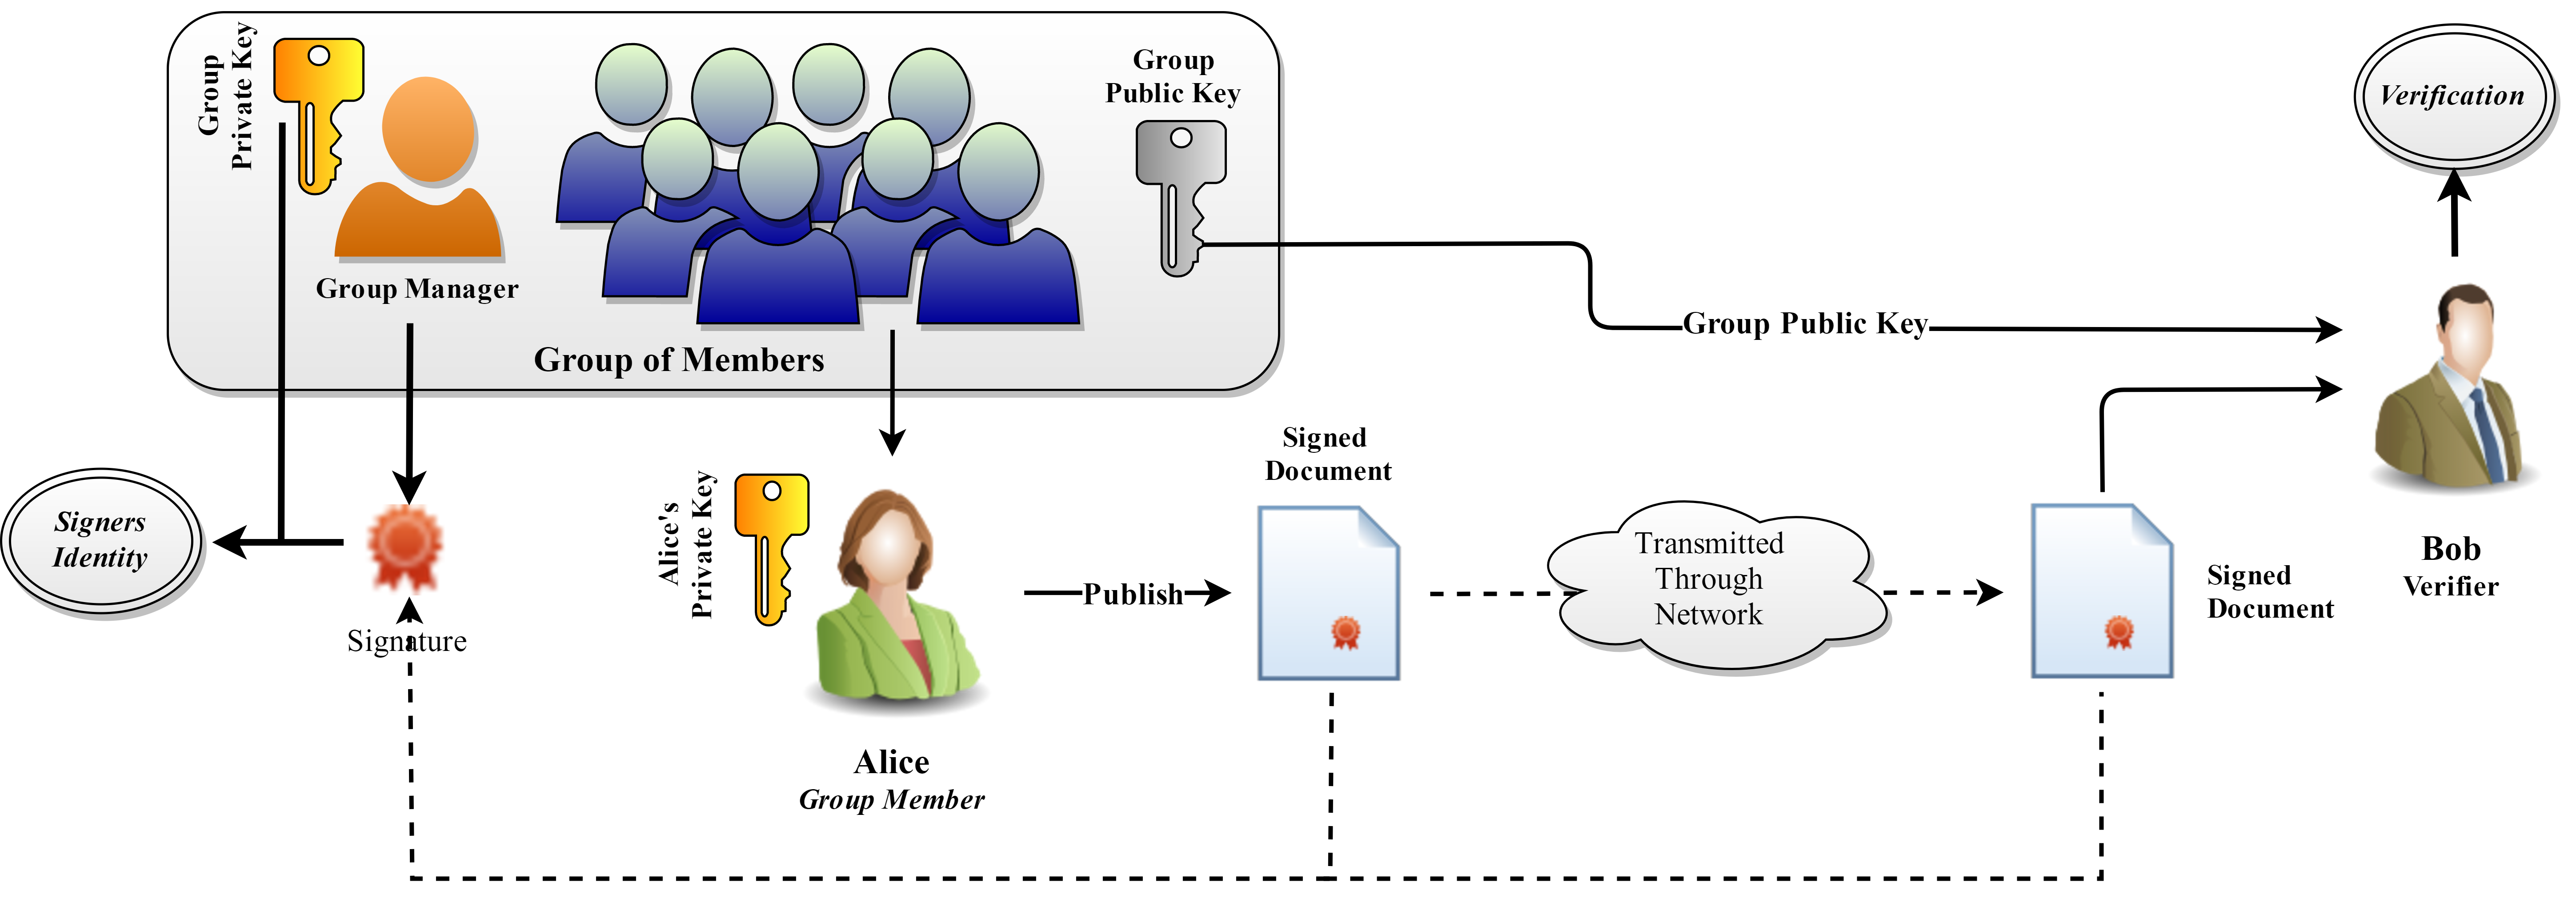
\includegraphics[width=\textwidth]{GroupSignature}
    \caption{Architecture of Group Signature }
    \label{fig:GroupSignature}
\end{figure}
\subsubsection{Group members}
The group member is the main beneficiary of the group signature scheme. The member joins the group by accepting a membership certificate which is required for obtaining private key of the member. After getting the membership certificate, a member can generate a signature for an arbitrary message. The signed message then transmitted to the receiver without disclosing the identity of the signer. The verifier of the message uses the public key of the group to verify issued group signature. 

The verification process proves that the signer is a valid member of the group, but the identity of the individual signer remains hidden from the verifier. Group Manager can open an issued signature. Therefore, it prevents any misuse of the power of anonymity and unlinkability provided to a member. The number knows that a disputed signature can be linked to its original signer.
\subsubsection{Verifier}
A verifier is an entity which authenticates the validity of a signature. To check the validity of a signature, the verifier uses the public key of the group, but the original signer of the signature cannot be known to a verifier. Instead, he only gets to know that the signer of the of a certain signature is a member of the group or not. No other information is known to the verifier. Therefore, he cannot extract information about any signer member.  

\subsubsection{Differences to PKI and Digital Signatures}
The group signature scheme appears similar to PKI-based authentication, but there is a significant variation between those two schemes. The Certificate Authority (CA) in PKI system, works similarly as Group Manager in group signature scheme. They both issues new certificate to users and have the ability to revoke the membership of a user. But the key difference between CA and Group Manager is that the certificate issued by CA contains the public key and some non-cryptographic information of the user where a certificate issued by Group Manager contains private key of the user and no other information. The certificate issued by CA is purposefully designed to be distributed publicly and the certificate issued by Group Manager must be retained secure and secret and should not be revealed by any group member.

The group signatures are different than the digital signatures in many ways. First, there is no public key required for group members whereas a public is needed for each user in the digital signature scheme. Instead, the group’s public key which is created by Group Manager is used for verification purpose and commonly used for verification of signatures, generated by all the group members. But still, the group signatures are publicly verifiable alike digital signatures.

The fundamental differences between ordinary signatures like digital signatures and group signatures is group signatures offer a guarantee of preserving the privacy of a user along with providing all the security services present in digital signatures. The public verification of group signatures does not leak any information of the signer during verification. The verifier authenticates signature based on information which only shows the status of membership of a signer, in the group. 

In group signatures, verifiers do not have the capability to recognize exact signer of a given signature. Instead, this ability is given to the Group Manager, which is a trusted authority. This unique combination of unlinkability and traceability not only gives signer the freedom to sign anonymously but also forces the responsibility of not misusing the power of anonymity. The misuse of a signature can be traced back to its original signer by   Group Manager, and sometimes the Group Manager can revoke the membership of such signer from the group. From above discussion, it can be seen that the group signatures provide greater functionality and applicability as compared to digital signatures.
\subsection{Security requirements of Group Signatures}
As the group signature provides authentication similar to digital signature it expected to provide all the security features available in the digital signature schemes. The group signatures are an enhancement to digital signatures required not only security features as of digital signatures but also some new specifications of its own, mainly due to the task of protecting the privacy of the signer. Several authors proposed these requirements for making the group signature scheme as secure as possible. All these requirements are needed to be proved correct by using mathematical basis and principals. A system implementing group signature must use number theoretical concepts not only to provide authentication but also to preserve privacy while following those security requirements. 
\subsubsection{Correctness}
Correctness\index{correctness} is the most fundamental property for group signature. The scheme having correctness property require always to generate a signature that can be verified correctly. That means legitimate signatures should have a negligible probability of identified as forged signature. The correctness property in a group signature can only be implemented by using mathematical proofs. There must be an accepted mathematical proof shows that the signing algorithm always creates such signatures which on verification gives accurate results and there is an only negligible possibility of false positive or negative.
\subsubsection{Unforgeability}
The unforgeability\index{unforgeability} property first introduced simultaneously with group signature scheme of D. Chaum \cite{chaum1991group}. It is similar to unforgeability of digital signatures. The unforgeability property permits only valid group member possessing a valid private key, to produce a legitimate signature and no one other can create such signatures. It is assumed that the private key of the signing member is safe and remain unknown to any attacker. The unforgeability property protects from chosen message attack in which an attacker might be able to produce valid group signature for a message selected from messages signed by a valid group member.
\subsubsection{Anonymity and Full Anonymity}
While proposing the first concept of group signature, D. Chaum considered anonymity\index{anonymity} to be a core property of group signature\cite{chaum1991group}. The anonymity requires that no one including verifiers of signature and other group members can be able to identify original signer of a signature, except for valid opening entity possessing a secret key. It implies that for a group of three members, a member who didn't sign, should not be able to identify which one of remaining two members was the signer of said signature. The property also assumes that the secret key for opening is secure and in possession of trusted authority who will not misuse it.

The strict model of Beller first introduced the concept of full anonymity\cite{bellare2003foundations}. The full anonymity\index{full anonymity} assumes that the private key of the signer is known to an attacker. And in such case too, it should not be possible to decide whether a given signature is from a particular signer or not. The main difference between anonymity and full anonymity is knowledge of private keys of a set of group members.
\subsubsection{Unlinkability}
The unlinkability\index{unlinkability} prevents to identifying any relation between two signatures. Beller introduces the unlinkability as a requirement for group signature\cite{bellare2003foundations}. The concept of unlinkability is associated to anonymity in some way. The unlinkability in group signature requires that it should not be possible to decide, whether two given signatures are from the same user or not. This property protects primarily from profiling attacks in which multiple messages from the same number are used for gathering information of members.
\subsubsection{Exculpability}
The concept of exculpability\index{exculpability} in group signature was introduced by Ateniese, as a variation of unforgeability\cite{ateniese1999some}. The requirement states that it should be impossible to create a valid signature for any member including Group Manager, which can be traced back to some other member. The exculpability defends a member from possible framing. When such property is present in group signature any signer can not be framed for signing a signature which he didn't sign. It also stops Group Manager from possible cheating and increases the trustworthiness of such authorities.
\subsubsection{Traceability}
The concept of traceability\index{traceability} was introduced while proposing the concept of group signature by D. Chaum\cite{chaum1991group}. The traceability is required for avoiding misuse of anonymity by the group members.  Any signature must be able to trace back to its original signer. The traceability also needed in following two scenarios. First, the group signatures cannot be able to produce a signature which gets verified as a legitimate but fails to identify its signer. Second, the tracing provides an output which is not the identity of the signer.
\subsubsection{Coalition Resistance}
Ateniese extends the traceability requirement for the group signature for resisting stronger attacks\cite{ateniese1999some}\index{coalition resistance}. This requirement checks that a colluding of multiple group member, should not be able to produce a valid signature by combining their keys. This requirement guarantees that a valid signature is always traceable to its one and only one signer. It also enhances the trust for the scheme and validity of a signature.
\subsubsection{Revocability}
The requirement of revocability\index{revocability} put a control on malicious nature of members. The revocability property enables the revocation of a member. Due to the implementation of this property, any member can be removed from the group at any time, and the signature produced by those member gets identified as invalid. The revocability puts a control on group member after they get their private key along with the power of creating anonymous signatures.
 
\subsection{Applications of Group Signatures}
The group signature has an enormous number of applications in real-world scenarios. The top applications of group signatures are in those scenarios where verifier does not require to know the actual identity of the signer. Instead, the knowledge of the membership status of the signer in an appropriate group is enough. Also, both the signer and verifier knows that the actual signer can be identified by trusted opening authority like Group Manager if needed.

Most beneficial utilization of group signatures can be found in conceal organizational structures like a company or government offices and administration. For example, an officer of government is trusted to issue orders, publish public statements, press releases, sign contracts and authorize financial transactions on account of the government. When group signatures used for this purpose, the actual identity of the officer will not be exposed, protecting him from revealing his identity to various parties involved in such matters. In this situation, the group signature not only protects the signing officer from threats or blackmailing but also helps to prevent corruption in the government.
However if such officer is found to be abusing his authority like signing illegal contracts or allowing illegal financial transactions, his identity can be revealed by using the Opening algorithm of the group signature. This opening can only be done by a trusted senior and high ranking officer so that the misuse of anonymous signing can be avoided. This opening procedure protects the organization from malicious employees to issue illegal documents or transactions. The opening of the signature can result in revocation of the signer, which can be achieved by the Revocation algorithm in group signature. The revocation algorithm not only eliminates the ability to produce valid signatures from the group member but also can be used to invalidate the valid signatures issued previously by the member.

Another application of group signatures is in online anonymous communication and identity escrow schemes. These schemes allow two parties to communicate anonymously. When a party misbehaves, its identity can be revealed by trusted opening entity. The group signature scheme can be converted to group identification scheme, where signature creation is transformed to the process of identification. This process of identification can be used to preserve the privacy of users, who identifies themselves to a third party. The paper of Lee explains the method of transformation of the group signature scheme to group identification scheme\cite{lee2010fiat}. This technique is useful in many circumstances, especially in outsourced service providing entities. An organization can acquire a service for its members, and members can utilize such service without giving their identity and just by using group identification scheme.

Some other applications of the group signatures are in electronic voting and bidding systems. In those schemes, a participant can place his bid anonymously without other parties identifying him. And when the auction concludes, the identity of winning party can be recognized by opening his signature. Some notable applications of group signature are in Vehicular Ad-Hoc Network (VANET)\nomenclature{VANET}{Vehicular Ad-Hoc Network} is proposed by Zhu et. el. where the identity of the vehicle is held secret while validating it\cite{zhu2013privacy}. The e-voting scheme of Lucas Malina can be used for implementing an electronic voting scheme where the identity of the voter can be kept secret and vote given by him cannot be linked to the voter\cite{malina2015secure}. 

The implementation of digital rights management can be achieved by applying group signatures. Group signature can be used for fingerprinting digital contents anonymously to protect the privacy of a user and still be able to identify the illegal distribution of such contents. 

This section proves that the group signature has infinite application in the real world, especially in the recent period where users are concerned with the preservation of their privacy, and service providers still need to authenticate the user.

\section{Motivation and Objective}
There are several approaches available which are able to provide authentication while protecting the privacy of the user. The group signature scheme is one of the best methods which provides a secure signing mechanism while protecting the privacy of the user by using the group based authentication approach. The digital signature scheme is found to be revolutionary in the digital documentation systems. Many modern documentation systems suffered from the problem of providing digital authentication before the emergence of the digital signature scheme. The digital signatures provide an efficient way to which the electronic documents can be signed and verified authentically, and it is impossible to replicate such signature to anyone except for the legitimate signer. While the digital signature solves the problem of digital authentication, it also issues concerns about the privacy of the signer.

In the paper based authentication system, the paper representing the message generally have signatures of the signer along with the seal of the signer. The seal is used to represent the position and power of the signer, but the advantages of the seal are they do not disclose any personal information about their holder. This approach protects the signer while providing the authentication because the signature alone contains very little information and the seal represents only the authority of the signer by which the verifier can assume that the signer possesses such authority to sign the document.

The digital signatures do not provide these kinds of features. Therefore all the information of the signer is always considered to be public. Also, a valid signature does not necessarily represent the authority of the signer. Therefore some issues left unsolved for the organizational structures like a company or government departments which are using the digital signature for digitally signing their documents.

The solution to such problems was provided by the approach of the group based authentication systems. The group based authentication can represent the authority of the members the combining and forming a group of people having similar or equal authorization. The group signature scheme uses a similar group based authentication system for signing the message. There are many group signatures schemes proposed which provide secure authentication with privacy, but many of these same have some drawbacks. A detailed discussion about some of these systems along with their shortcoming will be discussed in the next chapter.

There is a lot of scopes available for improvement of the group signature schemes. These improvements consist of improving correctness of the signatures, reduction of the computational time and cost for generation of the signature, dynamic addition as well as revocation of the group members. The enhanced distribution of the trusted authorities and an efficient correlation between them and provision of a verifiable proof which can verify the actions of these authorities are also some additional improvement required. These domains of the group signature scheme should be improved so that the group signature scheme should become robust and secure.

The objective of this dissertation is to find an efficient distribution of the trusted authorities so that the users of the group signature system does not need to put all their faith in a single authority. Also replacing the trusted tasks of the authorities with mathematical approved algorithms can reduce the requirement of the trust in the trusted authorities. The revocation mechanism is the important but least discussed topic in the group signature scheme. The implementation of revocation supporting scheme with not only required to be efficient but also secure and robust is also one of the objectives. 

The computational cost of the implementing group signature scheme is expected to be lower for better efficiency. Therefore the reduction of computational time and space in the implementation of a secure and efficient group signature scheme is also one major objective of this dissertation. 

\section{Organization}
The work of the dissertation presents an architecture for dynamic groups signature scheme with distributed authorities and supporting the dynamic revocation of the group members. The group signature scheme also reduces the computational cost for generating the signature. The organization of rest of this dissertation is in the following manner.
\subsubsection{Chapter 2}
Chapter 2 presents background information about the group signature schemes which include the classification of groups signatures schemes according to their architecture. The chapter to describes various groups signature schemes proposed earlier with a review of their advantages and shortcomings. These schemes are described on the basis of their mathematical assumptions. The chapter also provides a short review of similar approaches presented earlier for providing authentication while preserving the privacy of the user.
\subsubsection{Chapter 3}
The Chapter 3 of this dissertation provides an introduction to some number theory concepts which are essential in cryptographic as well as group signature systems. The chapter provides the formal definition of the groups, trapdoor permutation, hash functions and random oracle model along with a brief description of number theoretical assumptions on which the proposed group signature scheme relies. It also provides some discussion about zero knowledge proofs and the signature of knowledge (SoK).
\subsubsection{Chapter 4}
Chapter 4 contains proposed work for this dissertation. The proposed work is broken into four sections. The distribution of authorities section shows how the authorities in proposed group signature scheme are distributed and their working.  In the next section we are providing the formal definition of proposed group signature scheme, and then the architecture of the system is introduced. The details of the algorithms and their customization with working is provided in the model development section.

\subsubsection{Chapter 5}
Chapter 5 of this dissertation provides the analysis of proposed group signatures scheme from the security as well as performance point of view. The chapter discusses the functionalities provided by the proposed group signature scheme and their advantages. Then the security properties of this scheme are analyzed, and the scheme is compared with some important group signature schemes. The performance analysis of the scheme discusses the complexity of the algorithms in it.

\subsubsection{Chapter 6}
Finally, the dissertation concludes in Chapter 6. The chapter provides the conclusion of the work in this dissertation along with the future scope of the proposed group signature scheme, and then the references used in this thesis are listed.